\section{Conclusion}\label{section_conclusion}
An interesting familiarity with this process occurs in neurological studies of sensory and motor processing in the human central nervous system.

\begin{figure}[!ht]
\centering
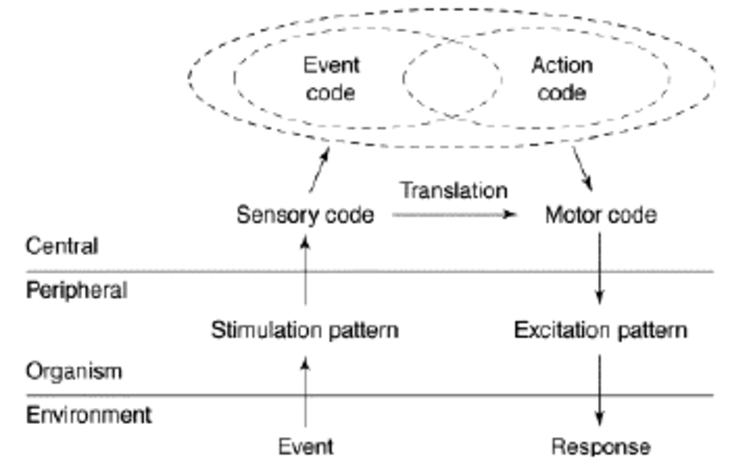
\includegraphics[width=0.5\textwidth]{images/neural-fig.pdf}
\caption{\label{neural-figure} Underlying neural mechanisms of sensory input to motor response.}
\end{figure}

\referenceFigure{neural-figure} demonstrates basic neural processes\footnote{Image Source: \url{http://www.sciencedirect.com}}
 associated with a change in the environment that are detected by human somatosensory signals to the brain, which are encoded and translated into motor signals that activate a motor response. The response is undoubtedly followed by a new change in environment and thus the cycle experienced with the PID controller system, is also observed in human everyday activity. This is one example of why it is so beneficial to acknowledge the similarities between both fields of study, where discoveries and advancements in one field may compliment or help advancements in the other. There is no doubt an obvious connection between human learning and machine learning, as machine learning is based on what we know of human neural processing, but identifying these connections is a helpful tool to understanding why things work the way they do or more importantly, why things aren't working the way they're expected to.
